\documentclass[border=6pt]{standalone}
\usepackage{tikz}
\usetikzlibrary{arrows.meta,decorations.pathreplacing}
\begin{document}
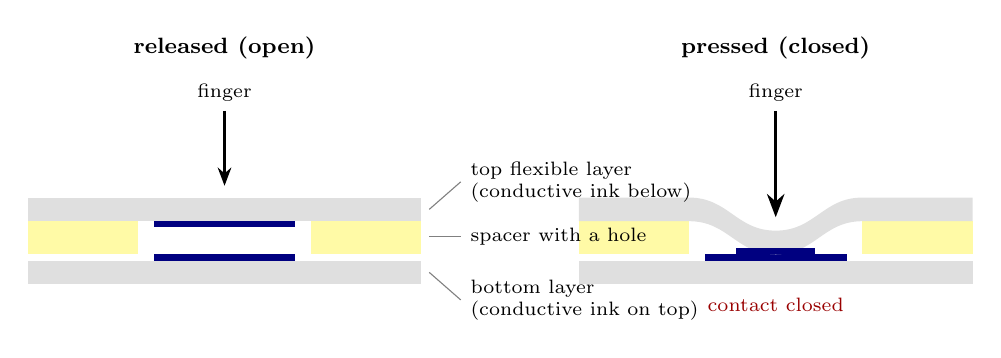
\begin{tikzpicture}[>=Stealth,font=\small]
% released key (left) and pressed key (right)
\foreach \dx/\t/\p in {0/released (open)/0,7/pressed (closed)/1} {
\begin{scope}[xshift=\dx cm]
\node[font=\footnotesize\bfseries] at (2.5,3.0) {\t};
% bottom layer
\fill[gray!25] (0,0) rectangle (5,0.3);
\fill[blue!50!black] (1.6,0.3) rectangle (3.4,0.38);
% spacer with a hole
\fill[yellow!35] (0,0.38) rectangle (1.4,0.8);
\fill[yellow!35] (3.6,0.38) rectangle (5,0.8);
\ifnum\p=0
  \fill[gray!25] (0,0.8) rectangle (5,1.1);
  \fill[blue!50!black] (1.6,0.72) rectangle (3.4,0.8);
  \draw[->,thick] (2.5,2.2) -- (2.5,1.25);
\else
  \fill[gray!25] (0,0.8) -- (1.4,0.8) .. controls (1.9,0.8) and (2.0,0.38) .. (2.5,0.38) .. controls (3.0,0.38) and (3.1,0.8) .. (3.6,0.8) -- (5,0.8) -- (5,1.1) -- (3.6,1.1) .. controls (3.1,1.1) and (3.0,0.68) .. (2.5,0.68) .. controls (2.0,0.68) and (1.9,1.1) .. (1.4,1.1) -- (0,1.1) -- cycle;
  \fill[blue!50!black] (2.0,0.38) rectangle (3.0,0.46);
  \draw[->,very thick] (2.5,2.2) -- (2.5,0.85);
  \node[font=\scriptsize,red!60!black,anchor=north] at (2.5,-0.05) {contact closed};
\fi
\node[font=\scriptsize,anchor=south] at (2.5,2.2) {finger};
\end{scope}}
% labels on the left picture
\draw[gray] (5.1,0.95) -- (5.5,1.3) node[right,font=\scriptsize,align=left,black]{top flexible layer\\(conductive ink below)};
\draw[gray] (5.1,0.6) -- (5.5,0.6) node[right,font=\scriptsize,black]{spacer with a hole};
\draw[gray] (5.1,0.15) -- (5.5,-0.2) node[right,font=\scriptsize,align=left,black]{bottom layer\\(conductive ink on top)};
\end{tikzpicture}
\end{document}
